\chapter{Implementation}

This chapter describes the theory behind the technical aspects of the prototype and how they were implemented into the prototype. This includes the necessary hardware to make the prototype and how these were used in conjunction with the software to make the prototype work. The software includes both the operations of the hardware and the musical processing of the input sounds.

\section{Theory}

This section explains the theory behind the effects that has been used in the implementation. 

\subsection{Pitch Shift}

The pitch shifter is built based on the principle of a rotating tape head, instead of using six tape heads as a machine would, the code uses two\citep{Katjaas_00}. The tape heads read the signal at a speed independent from the tape speed, thus the speed of the tape determines the duration of the sound and the direction of tape heads control the pitch shift. When the head rotates in the same direction as the tape, the pitch is lowered and if it rotates in the other direction, the pitch is increased, as seen in figure \ref{TapeHead}. \\

\begin{minipage}{\linewidth}% to keep image and caption on one page
\makebox[\linewidth]{%        to center the image
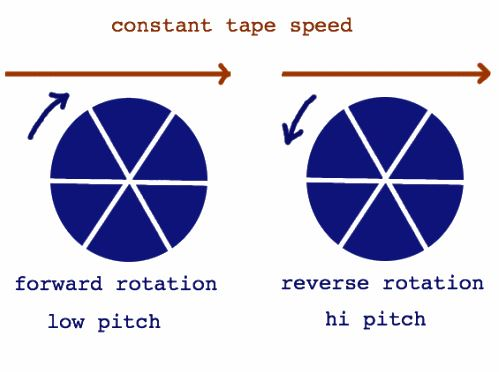
\includegraphics[keepaspectratio=true,scale=1]{TapeHead}}
\captionof{figure}{Graphical Impression of the tape head principle\citep{Katjaas_00}}\label{TapeHead}
\end{minipage}\\

In a digital setting the tape heads are replaced with two read pointers that change their delay depending on the required pitch shift. Increasing the delay when lowered pitch is needed and decreasing it if a raised pitch is needed. 
The read pointer will at some point pass the write pointer, because of the delay. When this happens a click can be heard if audio from only one read point is played. To combat this the cos~ object is used which creates a smooth crossfade to the second read pointer.

\subsection{Harmonise}

A harmony is a sound created by playing or singing different notes at the same time\citep{Harmonise02}.
Singing harmony means that a backup vocalist or someone else is singing the needed notes in conjunction with the lead singer singing the main melody notes. In a digital setting this effect can be achieved with a single voice. This is done by pitch-shifting the voice multiple times, each time with a different shift in semitones and stacking them together creating the effect of singing in harmony. Each of the harmonies is a chord made from major scale notes.
The notes are combined into threes and played at the same time. There are near infinite amount of ways to combine notes into groups of three, but by far the most popular way is triads\citep{Harmonise01}. Triad is a chord built on thirds, triad consists of root note, third and fifth, third being a third above root and fifth being a third above third. Depending on the quality of the two third intervals the quality of the triad changes. \\
In western music there are seven main harmonies, three major, three minor and one diminished. The quality varies between major, minor, diminished and augmented, the most popular ones being major and minor which will be the ones implemented in the program. The harmonise effect in the system is based on one minor and one major harmony and will allow the user to switch between those.

\section{Making the Prototype}

This section describes the hardware for the system and how it was made into a working prototype. This includes both the schematic, which explains how the system is put together, and the software for the prototype which both covers the software for the Arduino and sensor, and how they work together with Pure Data to process the input sounds for both harmonizing and pitch shift.

\subsection{Hardware}

The prototype consists of an Arduino Mega 2560\citep{Arduino}, with a connection to a circuit board with an inertial measurement unit(IMU). 
The IMU uses the MPU 9150 sensor with 9 degrees of freedom\citep{MPU}. It has a tri-axis gyroscope, magnetometer, and accelerometer.

\subsubsection{Schematic}

The following figure \ref{schematic} shows the connection from the Arduino to the circuit board with the IMU. The black switch at the top of the circuit board
represents the three connections, which is put on the thumb, index and middle finger. These are velcro based, with copper tape on them, to create the connection when pressed together. \\

\begin{minipage}{\linewidth}% to keep image and caption on one page
\makebox[\linewidth]{%        to center the image
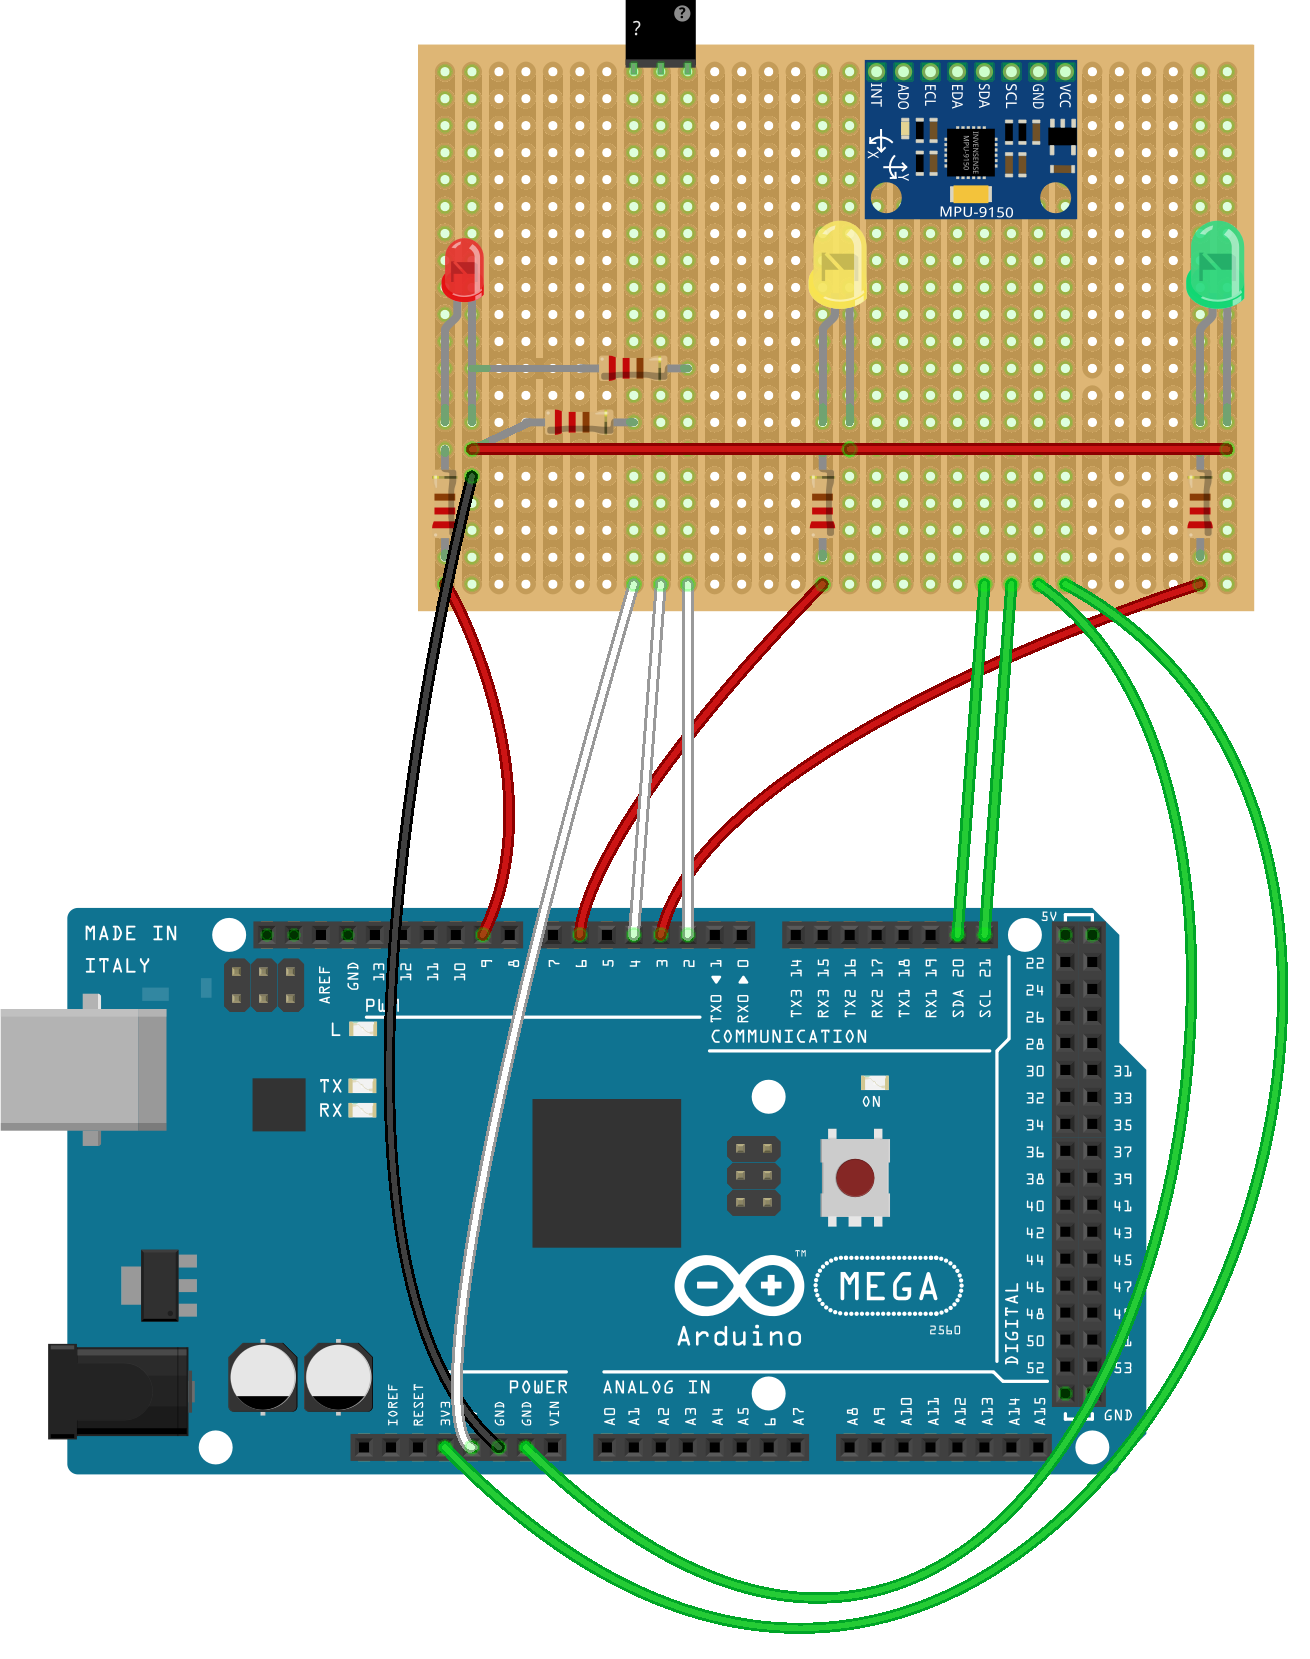
\includegraphics[keepaspectratio=true,scale=1]{Imu_Glove_Schematic}}
\captionof{figure}{Prototype Schematic}\label{schematic}
\end{minipage}\\

The circuit board consists of three LEDs, a yellow, green and red. They light up at different points, which is explained in the next section of this chapter.
The LEDs are connected to resistors of 220 Ohm, which are wired to the Arduino as seen in the schematic. The green LED is connected to pin 3. 
The yellow LED is connected to pin 6 and the red is connected to pin 9. This is essential to make it work in the Arduino code, which will be described later. 
The red wire connects all the LEDs and the black wire runs to the ground(GND) on the Arduino. The little blue circuit board on the yellow board represents the IMU. The necessary connections are: SDA, SCL, GND and VCC. 
SDA is the data line that sends data between the two devices, and the SCL is the clock line that sends pulses at a regular interval\citep{Arduino_SDA}. Every time the SCL changes from low to high, a single bit of information is send over the SDA.
The SDA connection is connected to pin 20 and the SCL is connected to pin 21. GND is connected to ground on the Arduino and the VCC connection powers the sensor and is therefore connected to 3.3V on the Arduino. The white wires are also connected to the Arduino. The first wire from the left, which goes to the thumb, is connected to the 5V on the Arduino. 
The white wire beside it, is connected to the index finger, and pin four on the Arduino. The last white wire is connected to the middle finger and pin two on the Arduino.
The wire which is connected to the thumb creates a circuit to the LEDs whenever the connection is created between either the thumb and index finger or thumb and middle finger. \\


The LEDs has to be connected to a pull-down resistor\citep{Pulldown_res}, which makes sure, that the Arduino does not 'float' between two different values. A pull-down resistor ensures, that the value is zero, when no active device is connected.
The following figure \ref{pull_down} shows how a circuit with a pull-down resistor might look. \\


\begin{minipage}{\linewidth}% to keep image and caption on one page
\makebox[\linewidth]{%        to center the image
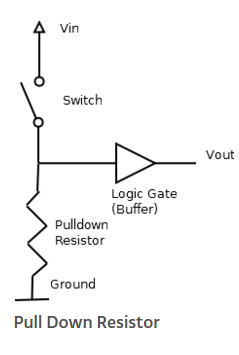
\includegraphics[keepaspectratio=true,scale=0.7]{Pull_down_resistor}}
\captionof{figure}{Schematic of Pull-down resistor\citep{Pulldown_res}}\label{pull_down}
\end{minipage}\\

Figure \ref{prototype} shows the prototype. As one can see, the velcro for the fingers has copper tape on it, which has been glued onto the velcro. The velcro enables the user to wear the glove, and use it properly.  
This means that whenever the copper tape gets connected with the copper tape on the thumb, it creates the connection as mentioned earlier. 
The prototype has cloth sewed onto it, which makes it possible to wrap it around the wrist. \\

\todo{Picture with front and back of prototype here}
%\begin{minipage}{\linewidth}% to keep image and caption on one page
%\makebox[\linewidth]{%        to center the image
%\includegraphics[keepaspectratio=true,scale=0.7]{Prototype}}
%\captionof{figure}{The front and back of the prototype}\label{prototype}
%\end{minipage}

\subsection{Software}

The following section describes the software part of the implementation. 

\subsubsection{Arduino}
The Arduino language is based on C/C++, and whenever a sketch is compiled, it is sent to a C/C++ compiler \citep{Arduino_FAQ}.\\

Information from the IMU is continually read and send to the Arduino program. This data is then calculated by the Arduino program. It gives the pose, the angle, and the current movement of the IMU. All based on the data from the gyroscope, accelerometer and magnetometer.

The first part of the code shown in figure \ref{index_finger} reads the state of the copper plates. The following if-statement is executed whenever the index finger is connected with the thumb. 
If the user turns the hand to the left, the code sends the information to PureData, and if the hand is turned to the right, it sends that information. 
The direction of the hand determines the pitch within a value of 0-255. The motion is a rolling motion, which resembles the motion of turning a knob. \\


\begin{minipage}{\linewidth}% to keep image and caption on one page
\makebox[\linewidth]{%        to center the image
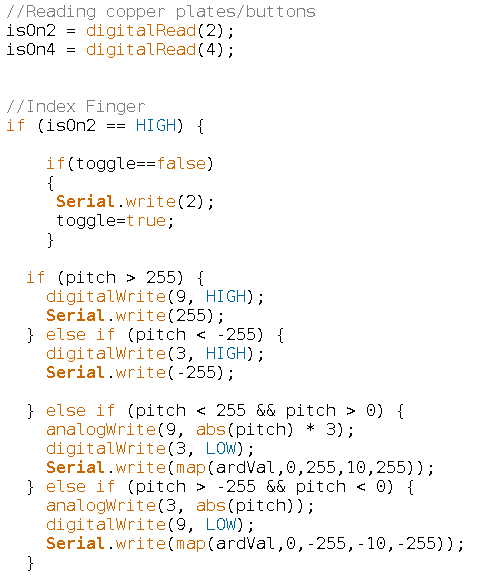
\includegraphics[keepaspectratio=true,scale=0.5]{Ardunio_Index_Finger}}
\captionof{figure}{Defining what happens when the index finger is connected}\label{index_finger}
\end{minipage}\\

The code used for the middle finger is almost identical. It does however use different pins. Initially it was the plan to use the raise/lower movement for the pitch shifting, but since it caused some errors, it was decided to use the rolling motion for pitch also.\\

Figure \ref{Arduino_else} shows the last part of the code. This is an else statement that makes sure that the button is off whenever the copper plate is released. 

\begin{minipage}{\linewidth}% to keep image and caption on one page
\makebox[\linewidth]{%        to center the image
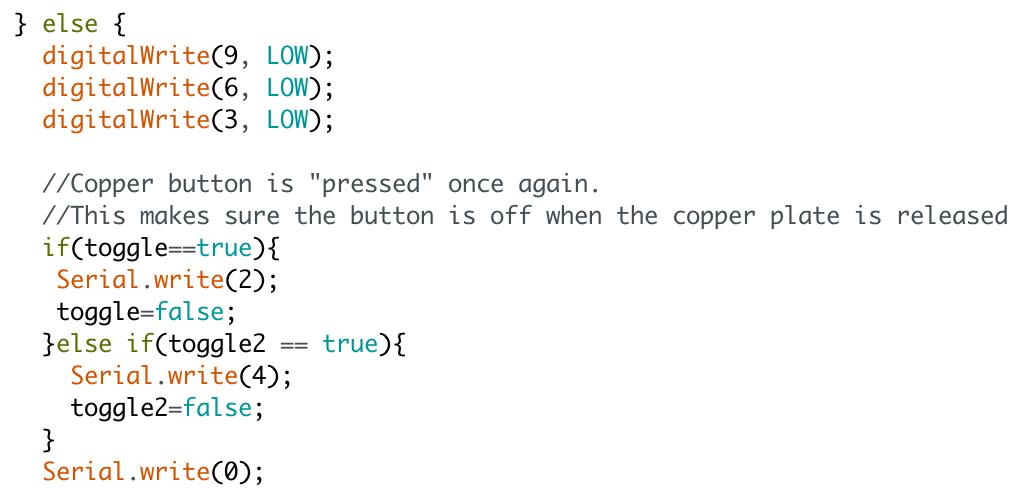
\includegraphics[keepaspectratio=true,scale=0.5]{Ardunio_else}}
\captionof{figure}{Else statement which makes sure the button is off when released}\label{Arduino_else}
\end{minipage}


\subsubsection{Pure Data}

The audio processing has been done in Pure Data(PD)\citep{PD_Info}, which is an open source programming language. It is used to generate and process sound, in a graphical way. 
The program uses patches where one can create objects which makes it possible to create different audio effects. The following subsection describes how PD has been used in this project, and explains the patches made for this project. \\

The following figure \ref{PitchShifting_PD} shows the pitch shifting patch made in PD. \\


\begin{minipage}{\linewidth}% to keep image and caption on one page
\makebox[\linewidth]{%        to center the image
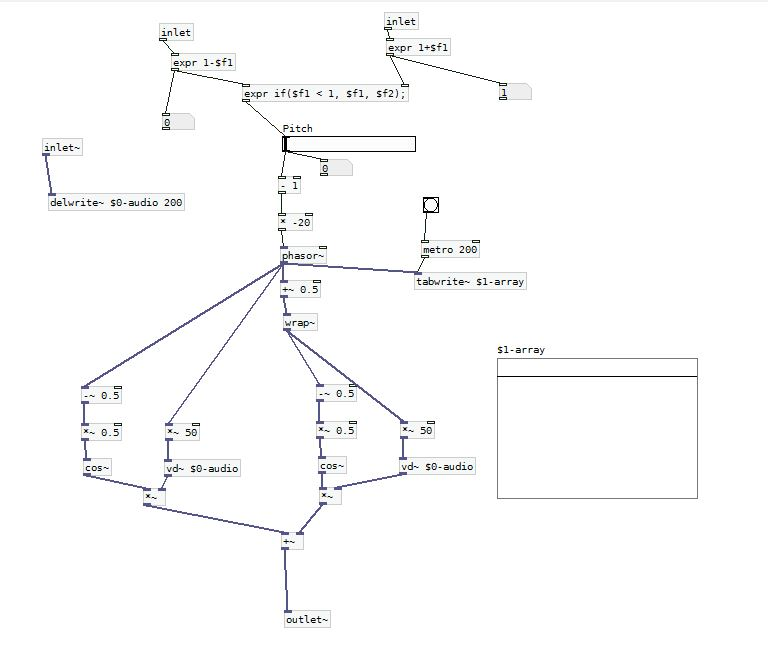
\includegraphics[keepaspectratio=true,scale=0.5]{PitchShifting_PD}}
\captionof{figure}{Pitchshifting in PureData}\label{PitchShifting_PD}
\end{minipage}\\

The patch uses the input, which might be coming from a microphone input. The slider called pitch shows how much the voice is actually being pitched. 

\section{Conclusion}

